\documentclass[a4paper, 11pt]{report}
\usepackage{graphicx}
\usepackage{xspace}
\usepackage[margin= 1in,includefoot]{geometry}
\newcommand\nth{\textsuperscript{th}\xspace}
\usepackage{xcolor}
\usepackage{lipsum}
\usepackage{listings}
\usepackage{amssymb} %maths
\usepackage{amsmath} %maths
\usepackage{mathptmx}
\begin{document}
\begin{figure}

\includegraphics[scale=.63]{medipol.png}
\centering
\end{figure}
\begin{titlepage}
\title{Introduction to Computer Engineering \\ Fall 2021, Assignment 5}
\author{by 64160010 - Rumeysa ÇELİK, Istanbul Medipol University}
\date{Due on Saturday December $25^{th}$, 2021 by 11:59 PM}
\maketitle
\end{titlepage}
{\center{\section*{{\textbf{Parameters Specific To Your Submission}}}}}
{\setlength{\parindent}{0pt}{In this assignment we will use the digits from your IDs. We define the following numbers
which are the \textbf{same} as the \textbf{numbers} you used in your assignment :}
\\ \\
$c_1$: The average of of digits from your student ID, \textbf{rounded} + 1. Use Excel file provided
to determine $c_1$.
\\ \\ My student ID is: 64160010
\begin{align*}
Average : \frac{6+4+1+6+0+0+1+0}{8} = \frac{18}{8} = 2.25 \approx 2 \\
c_1 = 2
\end{align*}
\\
$c_2$ : The average of digits from your Turkish ID, \textbf{rounded} + 1. Use the Excel file to determine $c_2$.
\\ \\
My Turkish ID is: 33098186424
\begin{align*}
Average: \frac{3+3+0+9+8+1+8+6+4+2+4}{11} = \frac{48}{11} = 4.36363636 \approx 4 \\
c_2 = 4
\end{align*}
\\
$c_3$: If $(c_1 \geq c_2)$ then $c_3 = 1$ otherwise $c_3 = -1$ .
\\ \\
$c_1 < c_2$ so that by $c_3 = -1$.
\\ \\
$c_4$ = $c_1$ + $c_2$.
\\ \\
Then,
\begin{align*}
c_4 = 2 + 4 = 6\\
c_4 = 6
\end{align*}
\\
$c_5$ : The first digit for your student ID.
\\ \\
My Student ID is: 64160010
\\ So that by $c_5$ = 6
\newpage
\section*{\textbf{Q1. Solve thefollowing two parts and show all the steps of your work(refer to slides 23-24 in Lecture 1)}}
\begin{itemize}
\item[(a)] Consider the following circuit. Find the final outputs for the four cases when the Twoinputs are 011, 110. Show all the intermediate results, that is draw four copies of this circuit and show your results on each of the four copies separately.
\begin{figure}[h]
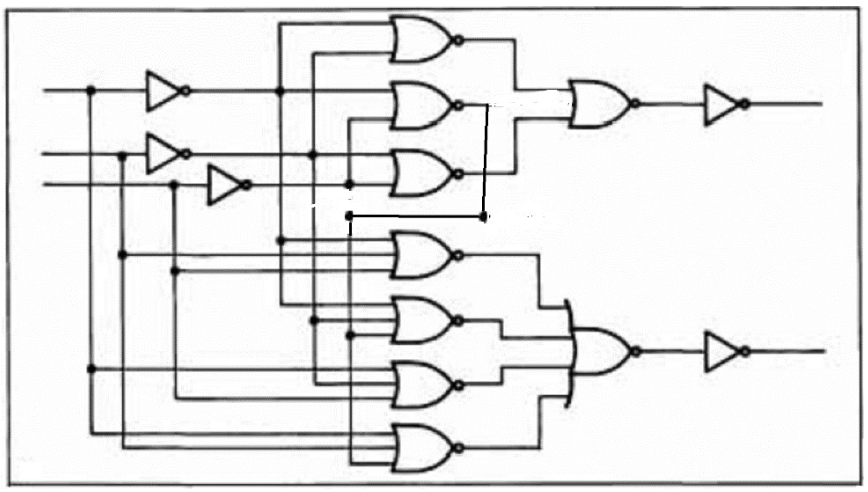
\includegraphics[scale=.63]{1.png}
\centering
\end{figure}
\end{itemize}


\end{document}
